\documentclass{article}
\usepackage{graphicx}
\usepackage{tikz}
\usetikzlibrary{intersections}
\usepackage{amssymb,amsmath}
\usepackage{hyperref}

\usepackage{fullpage}
\usepackage[parfill]{parskip}

%\setlength{\parindent}{0cm}


\title{PCUTL peer review: Description of feedback mechanisms}
\author{Vincent Knight}
\date{}

\begin{document}

\maketitle

\section{General discussion about feedback}

I have chosen to make feedback the focus of this peer review.

I practice a pedagogic approach based upon a flipped classroom approach. This approach ensures a continuous feedback loop between myself and my learners.

In Figure \ref{flipped_classroom_diagram}, a diagrammatic representation of a flipped classroom is given, showing that contact time is spent continuing to construct the learning of the students and also allowing me to obtain and importantly give feedback as to their ongoing development.

\begin{figure}[htdp]
\begin{center}
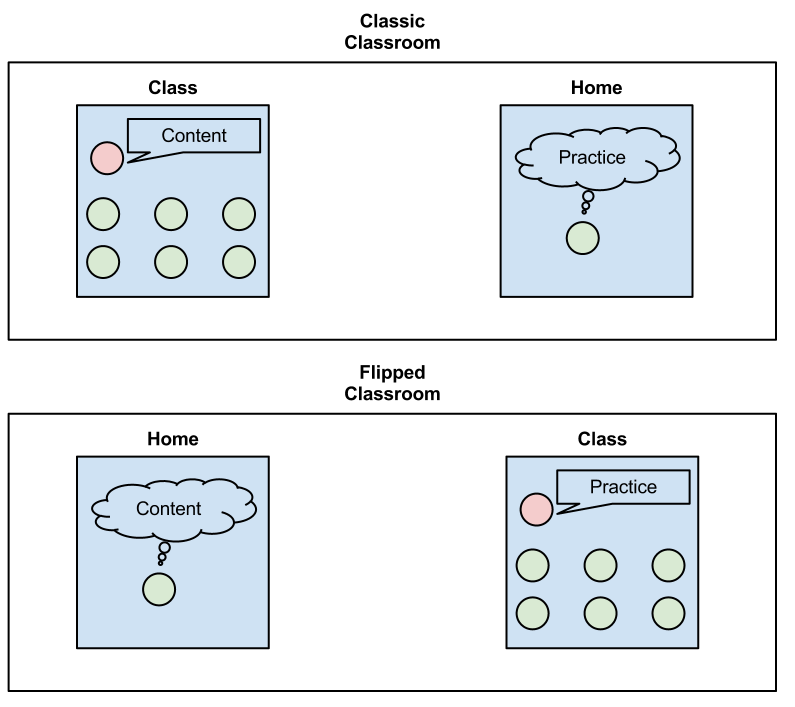
\includegraphics[width=10cm]{./Images/flipped_classroom_diagram.png}
\end{center}
\caption{A diagrammatic representation of a flipped classroom}\label{flipped_classroom_diagram}
\end{figure}

I will return to this aspect in the next section as feedback and flipping classrooms is a major aspect of a new module (core first year module) I am running for the first time. However I thought I would also discuss some traditional feedback mechanisms I continue to use.

Figure \ref{writtenfeedback} shows some written feedback I have given to students in the past (the entire class test is attached). This was feedback given for a programming class test for MAT013. In the feedback I point out the errors made by students and what would have needed to have been done to obtain a better mark.

\begin{figure}[htdp]
\begin{center}
\includegraphics[width=10cm]{./Images/writtenfeedback.pdf}
\end{center}
\caption{Some written feedback}\label{writtenfeedback}
\end{figure}

In the next section I will discuss a new module: MA1003 which has been the main focus of my PCUTL portfolio, concentrating on the feedback aspects of the module.

\section{Discussion about Computing for Mathematics}

This new module is designed using a completely flipped pedagogy. Students obtain content for a particular topic prior to the lecture on that topic. This content is delivered using a combination of written lab sheets and videos. An example of this can be seen here: \url{http://drvinceknight.github.io/Computing_for_mathematics/LabSheets/Week_02.html}.

Figure \ref{CfMdelivery} shows the content delivery, assessment and feedback for MA1003 (this is in fact only shown for the first half of the module).

\begin{figure}[htdp]
\begin{center}
\framebox{
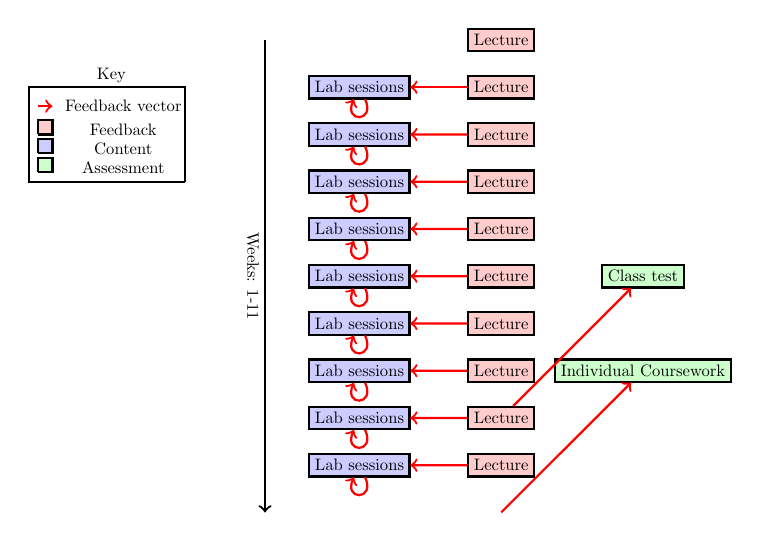
\begin{tikzpicture}[thick,scale=0.6, every node/.style={scale=0.6}]
\begin{scope}[xshift=-3cm, yshift=-3cm]
    \node at (-2.25, 3.25) {Key};
    % Color key
    \draw (-.7, 1) -- (-4, 1) -- (-4, 3) -- (-.7, 3) -- (-.7, 1);
    % Feedback
    \draw [fill=green!20] (-3.8, 1.2) -- (-3.8, 1.5) -- (-3.5, 1.5) -- (-3.5, 1.2) -- (-3.8, 1.2);
    \node at (-2, 1.3) {Assessment};
    % Content
    \draw [fill=blue!20] (-3.8, 1.6) -- (-3.8, 1.9) -- (-3.5, 1.9) -- (-3.5, 1.6) -- (-3.8, 1.6);
    \node at (-2, 1.7) {Content};
    % Assessment
    \draw [fill=red!20] (-3.8, 2) -- (-3.8, 2.3) -- (-3.5, 2.3) -- (-3.5, 2) -- (-3.8, 2);
    \node at (-2, 2.1) {Feedback};
    % Feedback direction
    \draw [red, ->] (-3.8, 2.6) -- (-3.5,2.6);
    \node  at (-2, 2.6) {Feedback vector};
\end{scope}
%------------ Weeks
\draw [->] (-2,1) -- (-2,-9) node [midway, below, rotate=-90] {Weeks: 1-11};


% ----------- Autumn
% Draw lab session boxes
\node (week2) [rectangle, draw, fill=blue!20] at (0,0) {Lab sessions};
\node (week3) [rectangle, draw, fill=blue!20] at (0,-1) {Lab sessions};
\node (week4) [rectangle, draw, fill=blue!20] at (0,-2) {Lab sessions};
\node (week5) [rectangle, draw, fill=blue!20] at (0,-3) {Lab sessions};
\node (week6) [rectangle, draw, fill=blue!20] at (0,-4) {Lab sessions};
\node (week7) [rectangle, draw, fill=blue!20] at (0,-5) {Lab sessions};
\node (week8) [rectangle, draw, fill=blue!20] at (0,-6) {Lab sessions};
\node (week9) [rectangle, draw, fill=blue!20] at (0,-7) {Lab sessions};
\node (week10) [rectangle, draw, fill=blue!20] at (0,-8) {Lab sessions};
% Draw Lecture boxes
\node (lec1) [rectangle, draw, fill=red!20] at (3,1) {Lecture};
\node (lec2) [rectangle, draw, fill=red!20] at (3,0) {Lecture};
\node (lec3) [rectangle, draw, fill=red!20] at (3,-1) {Lecture};
\node (lec4) [rectangle, draw, fill=red!20] at (3,-2) {Lecture};
\node (lec5) [rectangle, draw, fill=red!20] at (3,-3) {Lecture};
\node (lec6) [rectangle, draw, fill=red!20] at (3,-4) {Lecture};
\node (lec7) [rectangle, draw, fill=red!20] at (3,-5) {Lecture};
\node (lec8) [rectangle, draw, fill=red!20] at (3,-6) {Lecture};
\node (lec9) [rectangle, draw, fill=red!20] at (3,-7) {Lecture};
\node (lec10) [rectangle, draw, fill=red!20] at (3,-8) {Lecture};
% Draw feedback arrows
\draw [red, ->] (lec2) -- (week2);
\draw [red, ->] (week2) to [out=-65, in=-115, looseness=6]  (week2);
\draw [red, ->] (lec3) -- (week3);
\draw [red, ->] (week3) to [out=-65, in=-115, looseness=6]  (week3);
\draw [red, ->] (lec4) -- (week4);
\draw [red, ->] (week4) to [out=-65, in=-115, looseness=6]  (week4);
\draw [red, ->] (lec5) -- (week5);
\draw [red, ->] (week5) to [out=-65, in=-115, looseness=6]  (week5);
\draw [red, ->] (lec6) -- (week6);
\draw [red, ->] (week6) to [out=-65, in=-115, looseness=6]  (week6);
\draw [red, ->] (lec7) -- (week7);
\draw [red, ->] (week7) to [out=-65, in=-115, looseness=6]  (week7);
\draw [red, ->] (lec8) -- (week8);
\draw [red, ->] (week8) to [out=-65, in=-115, looseness=6]  (week8);
\draw [red, ->] (lec9) -- (week9);
\draw [red, ->] (week9) to [out=-65, in=-115, looseness=6]  (week9);
\draw [red, ->] (lec10) -- (week10);
\draw [red, ->] (week10) to [out=-65, in=-115, looseness=6]  (week10);
% Highlight assessment
\node (ass1) [rectangle, draw, fill=green!20] at (6,-4) {Class test};
\node (ass2) [rectangle, draw, fill=green!20] at (6,-6) {Individual Coursework};
% Feedback loops for assessment
\draw [red, ->] (lec9) -- (ass1);
\draw [red, ->] (3, -9) -- (ass2);
\end{tikzpicture}
}
\end{center}
\caption{Delivery of content, feedback and assessment for MA1003}\label{CfMdelivery}
\end{figure}

There are various aspects of feedback that need to be discussed for the purpose of this peer review:

\begin{itemize}
    \item \textbf{Feedforward}

    First of all, the flipped approach allows for the videos used to serve as not only delivery content but also feed forward mechanisms as to how to carry out a particular piece of assessment correctly. This video: \url{http://www.youtube.com/watch?v=7KxOxWC3h78} gives some feedback to students on a previous exercise whilst indicating what they must pay attention to in the current exercise.

    \item \textbf{Feedback in each lab}

    In each lab session tutors use a very `swift' feedback mechanism called `tickables'. This allows for the student to get immediate feedback as to whether or not they managed a particular task. This allows the tutors to gain an understanding of what difficulties were common on a given task.

    \item \textbf{Feedback in lecture}

    Gathering information as to what students were having difficulty with allows the lecture to be feedback focused. I address particular aspects that students found difficult.

    \item \textbf{Feedback in Office hours}

    Finally, I have started official use of `office hours' so that students can seek feedback from me on a 1 to 1 basis.
\end{itemize}

The above feedback mechanisms not only fit naturally within a flipped classroom but also (thanks to the tickables) allow for each student to have some level (often very brief) of individual feedback on each task every week. I'm not sure that with a class of this size (165 students) that would be possible otherwise.
\end{document}
